% Overview:
%   COBASI TeX subfile for the project.
%   Each subfile MUST start with the following line
%		\documentclass[../main.tex]{subfiles}

\documentclass[../main.tex]{subfiles}

\begin{document}

\subsection{COBASI}
\label{cobasi}
 
È chiaro che quando le read sono allineate ad un genoma di riferimento, è necessario tollerare un certo grado di discrepanza, poiché la variazione non verrebbe rilevata utilizzando solo allineamenti perfetti. D'altra parte, a causa della struttura altamente ripetitiva e complessa del genoma umano, la tolleranza dei disallineamenti potrebbe comportare lo spostamento errato di alcune read, introducendo false varianti. \cite{gomez-romero2018cobasi} per affrontare questo apparente paradosso hanno applicato un approccio diverso al problema della rilevazione di SNV nei genomi umani, chiamato individualizzazione contestuale dei nucleotidi e ibridazione genomica virtuale, COIN-VGH; esso si basa su allineamenti perfetti di \textit{k}-mer unici delle read sul genoma di riferimento. Nonostante il successo nell'eliminazione di chiamate false positive rispetto ad approcci alternativi, COIN-VGH presenta importanti limiti: (1) può essere utilizzato solo nelle regioni aploidi del genoma, (2) richiede read relativamente lunghe e (3) impiega molto tempo,  utilizzando una grande quantità di RAM e archiviazione su disco.

Alla luce di questi problemi, \cite{gomez-romero2018cobasi} propongono COBASI, il quarto metodo che andremo ad analizzare, il quale si basa sull'approccio di COIN-VGH e può essere utilizzato per chiamare varianti da entrambe le regioni, aploide e diploide, del genoma umano e lavora sulle letture di sequenze brevi di seconda generazione con una coverage di 30 volte maggiore o più (durante i test, è stato usato un set di dati con una coverage fino a 100 volte maggiore). Oltre a superare le precedenti limitazioni di COIN-VGH, l'approccio proposto da COBASI è particolarmente adatto per identificare SNV \textit{de novo} attraverso l'analisi congiunta di dati di sequenziamento di trio genitori-figlio. A questo fine, utilizza solo corrispondenze perfette tra le read uniche e un genoma di riferimento. A partire dalle corrispondenze perfette, genera una rappresentazione della coverage per nucleotide delle read lungo il genoma e gli SNV \textit{de novo} vengono individuati come cambiamenti significativi nella coverage, potendo essere identificati con alta precisione.  


\subsubsection{Algoritmo}

COBASI estende l'analisi delle COIN-Strings (CS)\footnote{\ È chiaro che, quando un singolo nucleotide viene cercato lungo il genoma, la posizione a cui appartiene non può essere determinata in modo inequivocabile. Se nella ricerca vengono incorporati due nucleotidi adiacenti, l'insieme delle posizioni possibili viene ridotto, sebbene rimanga piuttosto ampio. Aumentandone la lunghezza, ad un certo punto, il contesto del nucleotide bersaglio conterrà abbastanza informazioni per determinare in modo inequivocabile la sua posizione. Premesso questo, viene definito COIN-String (CS) l'insieme di tutti i \textit{k}-mer sovrapposti (con una finestra scorrevole di un nucleotide) che sono localizzati in modo univoco. Pertanto, ogni nucleotide del genoma di riferimento è contenuto al massimo in \textit{k} CS.} per trovare in modo robusto variazioni nel campione analizzato all'interno del genoma. Quando un SNV è presente all'interno di un campione, in una particolare posizione X, si prevede che, per SNV eterozigoti circa la metà delle read o, per SNV omozigoti quasi tutte le read che si sovrappongono a X contengano la variazione. Di conseguenza, le CS che includono X saranno presenti solo nelle read che non contengono l'allele alternato. Questo può essere tradotto in pattern specifici, nominati regioni di firma di variazione (VSR). Una volta identificate le regioni candidate, gli allineamenti locali tra le letture e il genoma permetteranno di capire la tipologia di variante. Partendo da questa intuizione, possiamo osservare la pipeline, proposta in Figura \ref{fig:cobasi}: l'algoritmo di COBASI si articola nei seguenti passi.

 \begin{figure}[h!]
	\centering
  	\captionsetup{justification=centering}
 	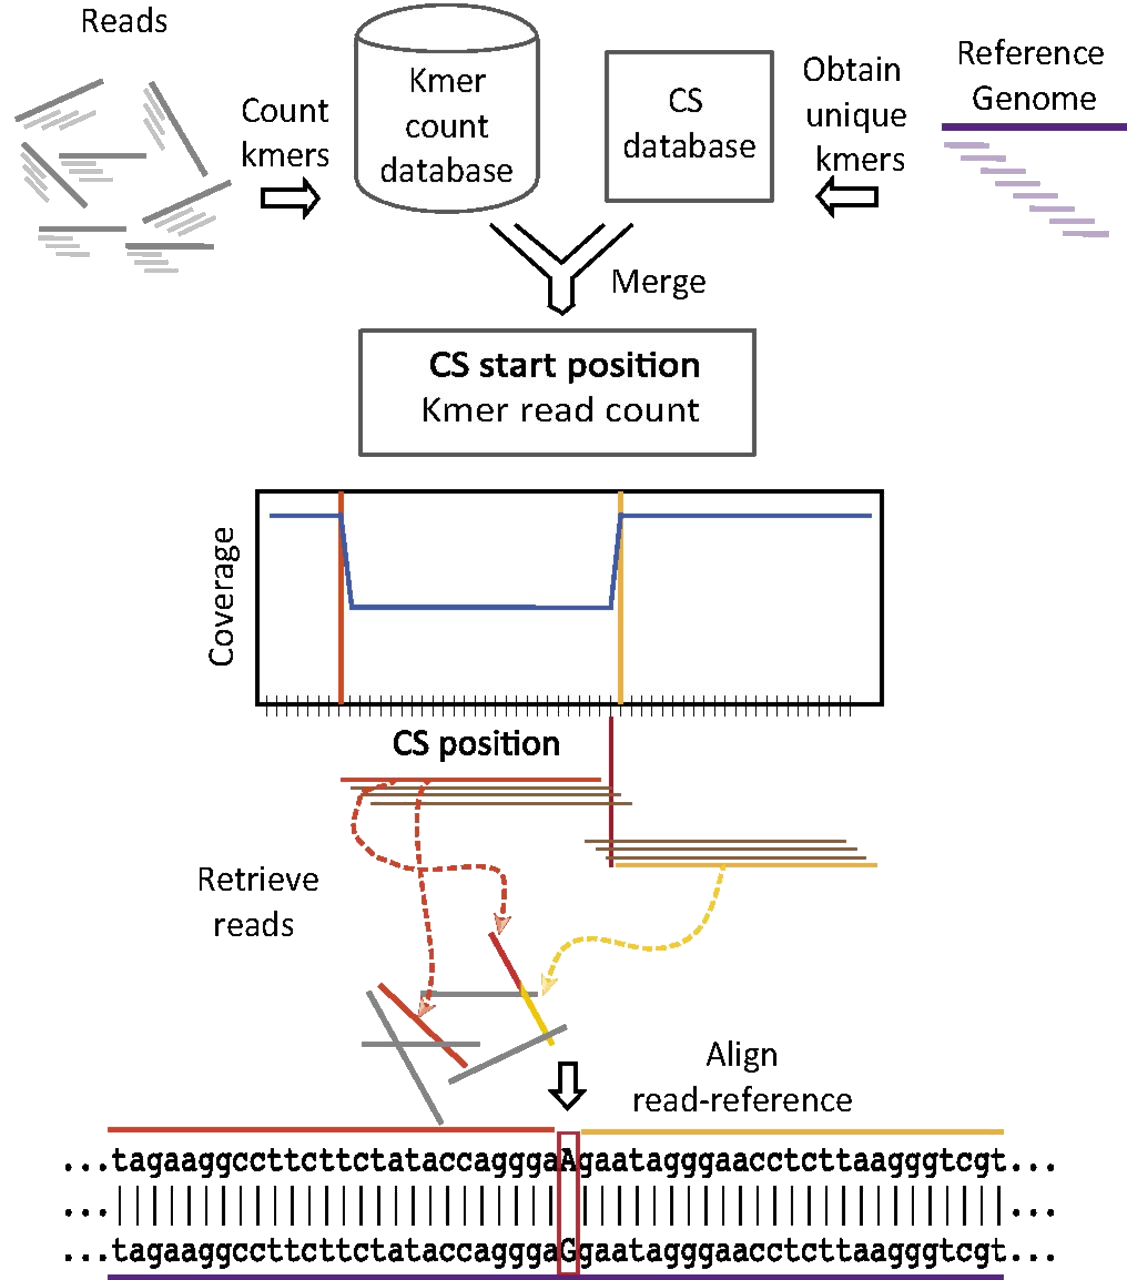
\includegraphics[scale=.15]{images/cobasi_pipeline.png}
  	\caption{Pipeline, COBASI.}
  	\label{fig:cobasi}
\end{figure}

\paragraph{Step 1} COBASI individua tutte le posizioni delle CS nel genoma accessibile\footnote{\ Viene definito \textit{genoma accessibile} da COBASI, l'unione di tutte le regioni lunghe almeno 100bp per le quali almeno il 50\% dei \textit{k}-mer ($k = 30$) contenuti al loro interno siano CS.}. Per fare ciò, genera tutte le finestre da 100nt (con una finestra scorrevole da 1bp) e per ciascuna finestra calcola il numero di CS tramite l'utilizzo del programma Jellyfish, il quale conta il numero di occorrenze di ciascun \textit{k}-mer lungo le read e scarta i \textit{k}-mer unici per evitare errori di sequenziamento. A questo punto, tutte le finestre consecutive con una densità di CS superiore a 0.5 sono concatenate, creando una regione di COIN-String accessibile. Queste regioni accessibili costituiscono il genoma richiamabile, ad eccezione dei \textit{k} nucleotidi all'inizio ed alla fine di ciascuna di esse.

\paragraph{Step 2} Vengono poi identificate e scartate le CS con una coverage anormale, utilizzando una coverage di soglia. Tale soglia corrisponde alla mediana dell'intervallo di coverage $\texttt{[+/-]10}$ interquartili (IQR), in quanto il $\sim$99,99\% delle CS presenta valori di coverage all'interno di questo intervallo. A questo punto, tramite i conteggi associati alle CS non scartate, viene generata la variation landscape, VL, una rappresentazione della coverage delle read che contengono ciascuna sequenza CS lungo l'intero genoma. Essa viene successivamente trasformata in RVL (relative variation landscape, per meglio definire la differenza di coverage tra due CS adiacenti) utilizzando un indice di coverage relativo (RCI), misurato su una scala da $\texttt{-1}$ a $\texttt{+1}$: l'RCI è vicino allo zero quando c'è poca o nessuna differenza nelle coverage, mentre il suo valore assoluto si avvicina a 1 quando si verificano brusche differenze, molto spesso a causa di una variazione generica. Poiché la RVL è variabile nelle regioni con coverage bassa, è stata stabilita una soglia di coverage per evitare errori nel processo di identificazione delle regioni di firma di variazione (VSR) parziali.

\begin{figure}[ht!]
	\centering
  	\captionsetup{justification=justified}
  	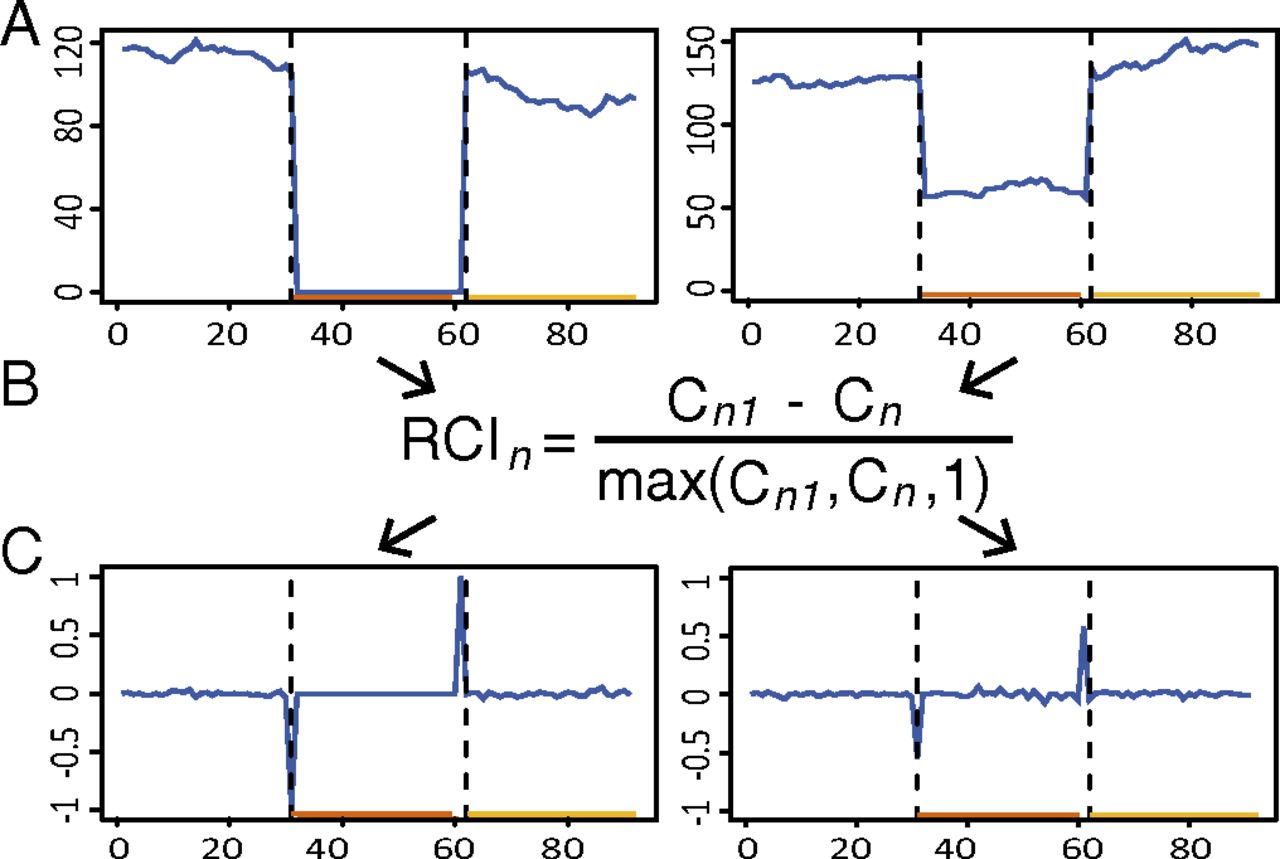
\includegraphics[scale=.80]{images/cobasi_rci.jpg}
  	\caption{Trasformazione di una VL in una RVL. A sinistra viene mostrato un SNV omozigote. A destra viene mostrato un SNV eterozigote. (A) Viene mostrata la VL per una regione composta da 30nt a monte e 30nt a valle di ciascuna VSR. I grafici mostrano la posizione iniziale di ciascun CS in quella regione genomica (asse x) e la copertura per ciascuna CS (asse y). (B) La VL viene trasformata in RVL utilizzando l'RCI. (C) La RVL per le stesse regioni mostrate in A. I grafici mostrano la posizione iniziale di ciascuna CS (asse x) e i valori RCI associati a ciascuna CS (asse y). La VL e la RVL sono rappresentate da linee blu. PrevCS e PostCS sono mostrati come linee arancioni e gialle nella parte inferiore di ogni grafico e le loro posizioni iniziali sono evidenziate con linee verticali nere tratteggiate. }
  	\label{fig:cobasi_rci}
\end{figure}

\paragraph{Step 3} Come anticipato, partendo dalle RVL, le VSR parziali possono essere identificate su tutte le mutazioni candidate. In particolare, COBASI cerca le regioni in cui la coverage subisce un brusco calo seguito da un brusco aumento. Queste VSR parziali sono estese alla maggior parte dei \textit{k} nucleotidi a monte e a valle della regione. Per caratterizzare drastici cambiamenti nella coverage, è richiesta una coverage minima e un valore assoluto minimo per l'RCI per ciascuna delle CS firma; definiamo come CS firma l'ultima CS prima dell'inizio di una VSR, chiamato PrevCS, e la prima CS dopo la fine di una VSR, chiamato  PostCS. In aggiunta, per estendere le VSR parziali, è stato stabilito un rapporto massimo tra la coverage di entrambi le CS firma. 

Vengono identificate le read contenenti corrispondenze perfette alle CS firma e vengono calcolati gli allineamenti globali tra la regione corrispondente nelle read e il genoma utilizzando la seguente strategia di allineamento: per ogni read, la regione dall'inizio di PrevCS alla fine di PostCS viene allineata alla regione corrispondente del genoma di riferimento: questi allineamenti sono considerati di alta qualità. Per le read contenenti solo PrevCS, l'allineamento tra genoma di riferimento e read è eseguito dall'inizio di PrevCS a 5nt a valle dell'ultimo nucleotide variante ottenuto dagli allineamenti di alta qualità. Poiché le CS sono garantite come uniche nel genoma e vengono prese in considerazione solo corrispondenze perfette, non sono richiesti ulteriori filtri di qualità. Inoltre per tutti gli allineamenti completi, sono stati identificati degli SNV.

\paragraph{Step 4} Per scoprire gli SNV \textit{de novo} nel genoma del figlio, le posizioni variabili al suo interno vengono interrogate nei genitori. Per ogni SNV nel figlio, le CS firma sono usate come ancore per recuperare le read di interesse nei genitori; le read dei genitori vengono quindi allineate al genoma di riferimento usando la procedura sopra descritta e viene generata una lista contenente tutti gli SNV del figlio e gli alleli trovati in ciascun genitore per le stesse posizioni. I genotipi di ogni SNV sono assegnati tramite opportune modifiche\footnote{\ Rispetto all'algoritmo presentato da Li, in \cite{gomez-romero2018cobasi} viene calcolata la probabilità dei tre possibili genotipi: riferimento omozigote (omo-R), riferimento eterozigote / nessun riferimento (ete-R / NR) e nessun riferimento omozigote (omo-NR). Se il genotipo assegnato è diverso da omo-R, l'allele con la più alta frequenza diversa dal riferimento è scelto ed è considerato l'allele maggiore. In aggiunta, sono calcolate tre probabilità: maggiore omozigote (omo-M), maggiore eterozigote / nessun maggiore (ete-M / NM) e nessun maggiore omozigote (omo-NM); se i genotipi con la più alta probabilità sono o omo-NR e omo-NM o ete-R / NR e ete-M / NM o ete-R / NR e omo-NM, allora ci sono almeno tre probabili alleli che possono essere assegnati con alta probabilità come genotipo in quel particolare sito e ciò comporta un'ambigua chiamata genotipica.} apportate all'algoritmo descritto in (Li, 2011, A statistical framework for SNP calling, mutation discovery, association mapping and population genetical parameter estimation from sequencing data.). Infine per identificare i potenziali SNV \textit{de novo}, vengono confrontati i genotipi di ciascuno degli individui del trio familiare, come si può vedere dalla seguente Figura \ref{fig:cobasi_align}.

\begin{figure}[ht!]
	\centering
  	\captionsetup{justification=centering}
  	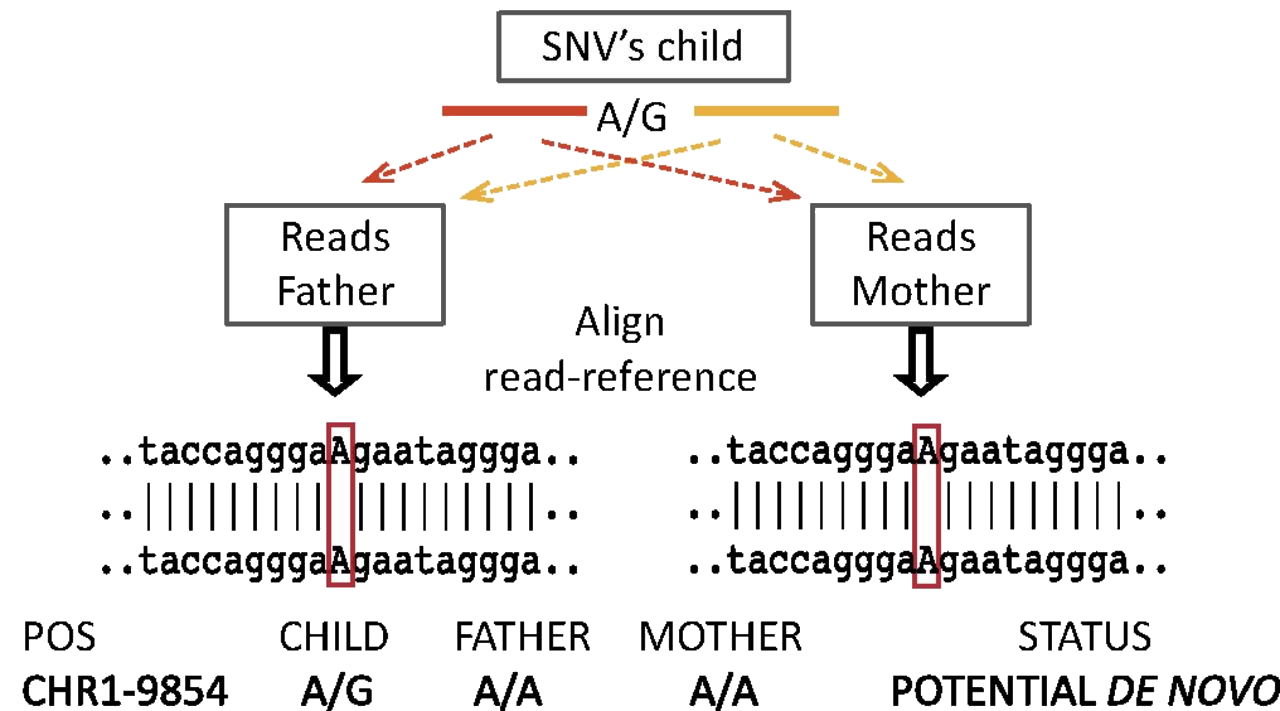
\includegraphics[scale=.20]{images/cobasi_align.png}
  	\caption{Confronti trio genitore-figlio}
  	\label{fig:cobasi_align}
\end{figure}

\noindent
\cite{gomez-romero2018cobasi} hanno definito i criteri per stabilire una possibile variante, come una variante in buona fede \textit{de novo}\footnote{\ I criteri per la definizione di una possibile variante come buona fede \textit{de novo} sono: (1) almeno 10 read che coprono quel sito nel bambino e in ciascun genitore e almeno 2 allineamenti totali nel bambino e in ciascun genitore, (2) l'allele variante non deve essere contenuto in più di un allineamento di alta qualità (allineamenti totali) in qualsiasi genitore (3) l'allele variante del bambino dovrebbe essere in più di un quarto di tutte le read che coprono quel sito o la regione della variante potrebbe essere duplicata in genoma infantile (4) il candidato SNV \textit{de novo} deve essere assente dai database SNV pubblici, come ad esempio dbSNP.}. Inoltre hanno constatato che esperimenti di sequenziamento con bassa coverage sono inclini a un numero più elevato di chiamate false negative e false positive. 

Pertanto, COBASI include requisiti di qualità aggiuntivi per evitare chiamate SNV \textit{de novo} errate e sono state identificate ed escluse le seguenti regioni soggette a errata assegnazione del genotipo: (1) regioni a bassa densità di CS, (2) regioni con più di una CS con una copertura superiore al previsto, (3) regioni con bassa copertura per una delle CS firma in qualsiasi individuo, (4) regioni con ulteriori significativi cambiamenti nella copertura all'interno della regione corrispondente alla VSR bambino: nel caso del bambino se si verifica un ulteriore calo o aumento, esso dovrebbe corrispondere a una regione quasi senza copertura, nel caso dei genitori, invece, non dovrebbe esistere alcun calo o aumento corrispondente alla posizione SNV del bambino e (5) regioni con una copertura disuguale in entrambi i lati della VSR per il bambino.

\end{document}